\documentclass[
  a4paper,uplatex,dvipdfmx,11pt,
  xcolor = {dvipsnames,svgnames},
  hyperref ={colorlinks=true,citecolor=Navy,linkcolor=NavyBlue,urlcolor=purple}
]{beamer}
\renewcommand{\baselinestretch}{1.4}

% ---refer `texdoc xcolor' at the command line---

% ---Display \subsubsection at the Index
% \setcounter{tocdepth}{3}

% ---Setting about the geometry of the document----
% \usepackage{a4wide}
% \pagestyle{empty}

% ---Physics and Math Packages---
\usepackage{amssymb,amsfonts,amsthm,mathtools}
\usepackage{physics,braket,bm}

% ---underline---
\usepackage{ulem}

% ---cancel---
\usepackage{cancel}

% --- surround the texts or equations
% \usepackage{fancybox,ascmac}

% ---settings of theorem environment---
% \usepackage{amsthm}
% \theoremstyle{definition}

% ---settings of proof environment---
% \renewcommand{\proofname}{\textbf{証明}}
% \renewcommand{\qedsymbol}{$\blacksquare$}

% ---Ignore the Warnings---
\usepackage{silence}
\WarningFilter{latexfont}{Some font shapes,Font shape}
\ExplSyntaxOn
\msg_redirect_name:nnn{hooks}{generic-deprecated}{none}
\ExplSyntaxOff

% ---Insert the figure (If insert the `draft' at the option, the process becomes faster.)---
\usepackage{graphicx}
% \usepackage{subcaption}

% ----Add a link to a text---
\usepackage{url,hyperref}
\usepackage{xcolor}
\usepackage{pxjahyper}

% ---Tikz---
\usepackage{tikz,pgf,pgfplots,circuitikz}
\pgfplotsset{compat=1.15}
\usetikzlibrary{intersections,arrows.meta,angles,calc,3d,decorations.pathmorphing,positioning}

% ---Add the section number to the equation, figure, and table number---
\makeatletter
   \renewcommand{\theequation}{\thesection.\arabic{equation}}
   \@addtoreset{equation}{section}
   
   \renewcommand{\thefigure}{\thesection.\arabic{figure}}
   \@addtoreset{figure}{section}
   
   \renewcommand{\thetable}{\thesection.\arabic{table}}
   \@addtoreset{table}{section}
\makeatother

% ---enumerate---
% \renewcommand{\labelenumi}{$\arabic{enumi}.$}
% \renewcommand{\labelenumii}{$(\arabic{enumii})$}

% ---beamer settings---
\usefonttheme{professionalfonts}
% \usefonttheme{serif}
\usecolortheme{seahorse}
\setbeamercolor{structure}{fg=white}
\setbeamercolor{local structure}{fg=Turquoise}
\setbeamertemplate{itemize item}[ball]
\setbeamertemplate{enumerate item}[circle]
\setbeamercolor{bibliography entry author}{fg=black}
\setbeamercolor{bibliography item}{fg=black}
\setbeamercolor{alerted text}{fg=RoyalBlue}
\setbeamertemplate{frametitle continuation}{}
\setbeamertemplate{footline}[frame number]
\setbeamertemplate{navigation symbols}{} 

% ---tcolorbox---
\usepackage{tcolorbox}
\tcbuselibrary{raster,skins}
\newtcolorbox{boxmine}[2][]{enhanced,
colframe=RoyalBlue!40!white,
colback=RoyalBlue!10!white,
coltitle=black,
drop fuzzy shadow, title={#2}
,#1}

% ---fonts---
\renewcommand{\familydefault}{\sfdefault}
\renewcommand{\kanjifamilydefault}{\gtdefault}
% \usepackage{newtxmath}
\mathversion{bold}

% ---citation---
\usepackage{usebib}
\newbibfield{author} 
\newbibfield{year} 
\newbibfield{journal} 
\newbibfield{doi} 
\bibinput{hoge}

\makeatletter
\newcommand*{\journal}{\begingroup\@makeother\#\@mylink}
\newcommand*{\@mylink}[1]{\href{http://dx.doi.org/\usebibentry{#1}{doi}}{\usebibentry{#1}{journal}}\endgroup} 
\makeatother

\newcommand*{\citefone}[3]{
  \begin{tikzpicture}[remember picture, overlay]
    \node[anchor=north east, align=left, text width=#3cm] at ($(current page.north east)-(0,0.0)$){
    {{\fontsize{5pt}{0pt}\selectfont
      \cite{#1}
      #2,
      \journal{#1}
      (\usebibentry{#1}{year}).\par}
    }
    };
  \end{tikzpicture}
}

\newcommand*{\citeftwo}[5]{
  \begin{tikzpicture}[remember picture, overlay]
    \node[anchor=north east, align=left, text width=#5cm] at ($(current page.north east)-(0,0.0)$){
    {{\fontsize{5pt}{0pt}\selectfont
      \cite{#1}
      #2,
      \journal{#1}
      (\usebibentry{#1}{year}).\par}

      {\fontsize{5pt}{0pt}\selectfont
      \cite{#3}
      #4,
      \journal{#3}
      (\usebibentry{#3}{year}).\par}
    }
    };
  \end{tikzpicture}
}

\newcommand*{\citefthree}[7]{
  \begin{tikzpicture}[remember picture, overlay]
    \node[anchor=north east, align=left, text width=#7cm] at ($(current page.north east)-(0,0.0)$){
    {{\fontsize{5pt}{0pt}\selectfont
    \cite{#1}
    #2,
    \journal{#1}
    (\usebibentry{#1}{year}).\par}

    {\fontsize{5pt}{0pt}\selectfont
    \cite{#3}
    #4,
    \journal{#3}
    (\usebibentry{#3}{year}).\par}

    {\fontsize{5pt}{0pt}\selectfont
    \cite{#5}
    #6,
    \journal{#5}
    (\usebibentry{#5}{year}).\par}
    }
    };
  \end{tikzpicture}
}


% ---Title---
\title{
  {\LARGE
    磁化トーラス上にコンパクト化した
    \\
    超対称模型におけるモジュライ固定
  }
}
\author{
  宮根 一樹
}
\date{2024年1月23日}



\begin{document}

\begin{frame}
  \titlepage
\end{frame}


\section{イントロダクション}

\begin{frame}
  \frametitle{\thesection.\ \secname}
  \citefone{Abe_AhlerModuli_2017}{H. Abe, T. Kobayashi, K. Sumita, and S. Uemura}{6}

  \vspace*{-20pt}

  高次元時空モデル:素粒子標準模型を再現する可能性

  \vspace*{-10pt}

  \begin{center}
    余剰次元は低エネルギーで\textcolor{DarkRed}{観測できないほど小さく}コンパクト化
  \end{center}

  余剰次元の大きさ(\textcolor{DarkBlue}{モジュライ})は力学的な場

  \vspace*{-10pt}

  \begin{flushright}
    $\rightarrow$低エネルギーで真空期待値に\textcolor{DarkBlue}{固定}    
  \end{flushright}

  \begin{boxmine}{本研究の動機}
    \centering
    標準模型の世代構造を再現する高次元時空モデル\cite{Abe_AhlerModuli_2017}で
    \\
    余剰次元の\textcolor{DarkBlue}{モジュライ}を\textcolor{DarkBlue}{固定}

    {\Large $\downarrow$}

    その値を用いて現象論的に興味のある量を計算
  \end{boxmine}

\end{frame}


\section{磁化トーラス模型}

\begin{frame}
  \frametitle{\thesection.\ \secname}
  \citefone{Abe_SuperfieldDescription_2012}{H. Abe, T. Kobayashi, H. Ohki, and K. Sumita}{6}

  \vspace*{-20pt}

  \uline{トーラスコンパクト化}

  4次元ミンコフスキー$+$\uwave{6次元余剰空間}

  余剰次元にトーラス$T^2$の境界条件$\rightarrow$コンパクト化
  
  \vspace*{-10pt}

  \begin{center}
    6次元
    $\rightarrow 
    T^{2}\times T^{2}\times T^{2}$
  \end{center}
  
  \vspace*{-20pt}

  \begin{equation}
    \mathcal{A}^{(i)}
    \text{
      :$i$番目のトーラスの面積
    }
    \nonumber
  \end{equation}

  \vspace*{-20pt}

  \begin{center}
    {\large $\downarrow$}
  \end{center}

  \vspace*{-20pt}

  \begin{center}
    $\ev*{T_{i}}=\mathcal{A}^{(i)}$となるような力学的な場
    $T_{i}$\textcolor{DarkBlue}{モジュライ}
  \end{center}

  \uline{背景磁場}:トーラスに背景磁場を導入  

  \vspace*{-10pt}

  \begin{flushright}
    $\longrightarrow$
    $\displaystyle
      B^{(i)}
      =
      \{
        M_{1}^{(i)},M_{2}^{(i)}
      \}
    $
    :
    $M_{a}^{(i)}$は整数    
  \end{flushright}

\end{frame}



\begin{frame}
  \frametitle{\thesection.\ \secname}

  \uline{モジュライのポテンシャル}
  \begin{equation}
    V^{(D)}(T_{i})
    =
    \sum_{a=1,2}
    \left(  
      \sum_{i=1,2,3}
      \frac{\pi M_{a}^{(i)}}{T_{i}}
    \right)^2
    \times
    \prod_{i=1,2,3}T_{i}
    \nonumber
  \end{equation}
  \begin{center}
    {\LARGE $\downarrow$}\ 真空期待値$\ev*{T_{i}}$の周りで展開
  \end{center}
  \begin{equation}
    V^{(D)}(T_{i})
    \sim
    V^{(D)}(\ev*{T_{i}})
    +
    \frac{1}{2}
    \underbrace{
      \partial_{T_{r}}\partial_{T_{r'}}V^{(D)}
      \left.\vphantom{\frac{1}{2}}\right|_{T_{i}=\ev*{T_{i}}}
    }_{\equiv V_{rr'}}
    \delta T_{r}\delta T_{r'}
    \nonumber
  \end{equation}

  \pause

  \uline{行列$V_{rr'}$の対角化}
  \begin{equation}    
    V^{D}
    \sim
    V^{(D)}(\ev*{\tilde{T}_{i}})
    +    
    \frac{1}{2}m_{2}^2 \delta \tilde{T}_{2}^2
    +
    \frac{1}{2}m_{3}^2 \delta \tilde{T}_{3}^2
    \nonumber
  \end{equation}
  \begin{center}
    $\tilde{T}_{i}$:対角化後の基底
    \ \&\ 
    $m_{2}^2,m_{3}^{2}$:$V_{rr'}$の固有値
  \end{center}
  
\end{frame}


\begin{frame}
  \frametitle{\thesection.\ \secname}
  \uline{新・旧基底の関係}\hspace*{3cm} $P$は対角化行列
  \begin{align*}
    &\ev*{T_{1}}
    =
    P_{11}\ev*{\tilde{T}_{1}}
    +
    P_{12}
    \only<1>{\ev*{\tilde{T}_{2}}}
    \only<2>{\cancel{\ev*{\tilde{T}_{2}}}}
    +
    P_{13}
    \only<1>{\ev*{\tilde{T}_{3}}}
    \only<2>{\cancel{\ev*{\tilde{T}_{3}}}}
    \\
    &\ev*{T_{2}}
    =
    P_{21}\ev*{\tilde{T}_{1}}
    +
    P_{22}
    \only<1>{\ev*{\tilde{T}_{2}}}
    \only<2>{\cancel{\ev*{\tilde{T}_{2}}}}
    +
    P_{23}
    \only<1>{\ev*{\tilde{T}_{3}}}
    \only<2>{\cancel{\ev*{\tilde{T}_{3}}}}
    \\
    &\ev*{T_{3}}
    =
    P_{31}\ev*{\tilde{T}_{1}}
    +
    P_{32}
    \only<1>{\ev*{\tilde{T}_{2}}}
    \only<2>{\cancel{\ev*{\tilde{T}_{2}}}}
    +
    P_{33}
    \only<1>{\ev*{\tilde{T}_{3}}}
    \only<2>{\cancel{\ev*{\tilde{T}_{3}}}}
  \end{align*}

  \onslide+<2>{
  $\rightarrow$モジュライ$\tilde{T}_{1}$の真空期待値が決まれば,$\ev*{T_{i}}$が全て決定

  \vspace*{10pt}

  \begin{boxmine}{今後の目標}
    \centering
    モジュライ$\tilde{T}_{1}\equiv\tilde{T}$の真空期待値$\ev*{\tilde{T}}$を決定
  \end{boxmine}
  }

\end{frame}


\section{モジュライ固定}

\begin{frame}
  \frametitle{\thesection.\ \secname}

  \uline{$\tilde{T}$のポテンシャル}

  スーパーポテンシャル$W$,ケーラーポテンシャル$K$
  \begin{align*}
    W
    &=
    w_{0}
    -
    A
    e^{-aP_{11}\tilde{T}}
    -
    Be^{-bP_{11}\tilde{T}}
    X
    \\
    K
    &=
    -
    3\ln (\tilde{T}+\bar{\tilde{T}})
    +
    |X|^2
  \end{align*}

  \vspace*{-15pt}

  \begin{center}
    {\LARGE $\downarrow$}
  \end{center}

  \vspace*{-8pt}

  \hspace*{-18pt}
  $\displaystyle  
    V^{(F)}(\tilde{T},X)
    =
    e^{K}
    (
      K^{I\bar{J}}(D_{I}W)(D_{\bar{J}}\bar{W})
      -
      3|W|^2
    )
  $:ポテンシャル

  \vspace*{-10pt}

  \begin{center}
    $
      f_{I}
      \equiv
      \partial_{I}f
      ,\ 
      D_{I}W
      \equiv
      W_{I}+K_{I}W
      \quad
      (I=X,\tilde{T})
    $
  \end{center}

  \vspace*{-10pt}

  \begin{flushright}
    $\rightarrow$最小点$(\ev*{T},\ev*{X})$は近似的に知られている    
  \end{flushright}

\end{frame}



\begin{frame}
  \frametitle{\thesection.\ \secname}
  \citeftwo{Abe_AhlerModuli_2017}{H. Abe, T. Kobayashi, K. Sumita, and S. Uemura}{Abe_ModuliStabilization_2007a}{H. Abe, T. Higaki, T. Kobayashi, and Y. Omura}{6}
  \uline{先行研究}\cite{Abe_AhlerModuli_2017,Abe_ModuliStabilization_2007a}
  \begin{align*}
    W
    &=
    \only<1>{
      w_{0}
      -
      Ae^{-aT}
      -
      Be^{-bT}
      X
    }
    \only<2>{
      w_{0}
      \tikz[baseline=(x.base)]{
            \node(x)[rectangle, fill=blue!10, rounded corners]{$\displaystyle
            -
            Ae^{-aT}
            -
            Be^{-bT}
            X$};
        }      
    }
    \\
    K
    &=
    -
    3\ln (T+\bar{T})
    +
    |X|^2
  \end{align*}
  
  \vspace*{-15pt}

  \begin{equation}
    w_{0}\ll 1,\ A,B\sim 1,\ a,b\sim 4\pi^2
    \nonumber
  \end{equation}

  \vspace*{-10pt}

  \begin{center}
    {\LARGE $\downarrow$}
  \end{center}

  \vspace*{-10pt}
  
  \begin{center}
    \textcolor{DarkRed}{
    $
      \displaystyle
      x
      =
      \sqrt{3}-1
      ,\ 
      t
      \only<2>{
        \ 
        \tikz[baseline=(x.base)]{
              \node(x)[rectangle, fill=blue!10, rounded corners]{$\displaystyle
              \sim 1.87$};
          } 
      }
      =
      \mathcal{O}(1)
    $    
    }

    \textcolor{DarkRed}{点$(t,x)$}は\textcolor{DarkBlue}{真の最小点$(\ev*{T},\ev*{X})$}の\textcolor{DarkRed}{近似点}

    $\rightarrow$以降はこの近似値を用いて計算
  \end{center}

  \onslide+<2>{
    \begin{tikzpicture}[remember picture, overlay]
      \draw[latex-latex](6.4,6.6)--++(0.5,0.5);
      \draw(6.9,7.1) node [above]{
        \small
        \uwave{今回のポテンシャル}
        :
        \tikz[baseline=(x.base)]{
            \node(x)[rectangle, fill=blue!10, rounded corners]{$\displaystyle
            -
            Ae^{-aP_{11}T}
            -
            Be^{-bP_{11}T}
            X$};
        }   
      };
    \end{tikzpicture}
  }

\end{frame}


% --------------------------


\section{計算結果}

\begin{frame}
  \frametitle{\thesection.\ \secname}

  \citeftwo{Abe_AhlerModuli_2017}{H. Abe, T. Kobayashi, K. Sumita, and S. Uemura}{Choi_PhenomenologyMixed_2005}{K. Choi, K. S. Jeong, and K. Okumura}{6}

  \vspace*{-20pt}

  \begin{center}
    (注:卒論 \& 発表までに改善)
  \end{center}

  磁場$M_{a}^{i}$の値を先行研究\cite{Abe_AhlerModuli_2017}の値にとる
  \begin{equation}
    M^{(1)}
    =
    \begin{pmatrix}
      7 & 0 \\
      0 & -7
    \end{pmatrix}
    ,\ 
    M^{(2)}
    =
    \begin{pmatrix}
      1 & 0 \\
      0 & 0
    \end{pmatrix}
    ,\ 
    M^{(3)}
    =
    \begin{pmatrix}
      0 & 0 \\
      0 & -1
    \end{pmatrix}
    \nonumber
  \end{equation}

  \uline{$M_{\text{Pl}}=1.2\times10^{19}\ \text{GeV}$を1にとる}

  \begin{itemize}
    \item 
    $
      \ev*{T_{1}}
      \sim
      1.907
      ,\ 
      \ev*{T_{2}},\ev*{T_{3}}
      \sim
      13.4
    $
    \item 
    $\displaystyle
      m_{2}^{(D)},\ m_{3}^{(D)}\sim 11
      ,\  
      m_{T}
      \sim
      10^{-29}
      \rightarrow m_{2}^{(D)},m_{3}^{(D)}\gg m_{T}
    $

    $\displaystyle
      F^{T}
      \sim
      10^{-46}
      \longrightarrow F^{T}\sim 0
    $
    \item 
    アノマリー伝播とモジュライ伝搬の比\cite{Choi_PhenomenologyMixed_2005}
    \begin{center}
      $
        \alpha
        \sim
        10^{13}
        \neq
        \mathcal{O}(1)
      $
    \end{center}
  \end{itemize}

\end{frame}


% --------------------------

\section{まとめと展望}

\begin{frame}
  \frametitle{\thesection.\ \secname}

  \uline{まとめ}
  \begin{itemize}
    \item 
    モジュライの真空期待値を決定$\rightarrow$余剰次元の大きさを決定
    \item 
    その値を用いて現象論的に興味のある量を計算
    \begin{itemize}
      \item 
      質量や超対称性は望ましい結果
      $\leftrightarrow$
      $\alpha$は望ましくない値
    \end{itemize}
  \end{itemize}

  \uline{展望}
  \begin{itemize}
    \item 
    モジュライ固定の計算

    \vspace*{-10pt}

    \begin{flushright}
      $\longrightarrow$今回は先行研究の計算をそのまま適用
    \end{flushright}
    \item 
    スーパーポテンシャルの形を変える
    \begin{itemize}
      \item 
      ブレーンによる非摂動効果を変化させた場合
      \item 
      ISS-KKLTモデルの場合
      \hspace*{4cm}
      など
    \end{itemize}
  \end{itemize}

\end{frame}

% --------------------------

\newcounter{Appendix}
\setcounter{Appendix}{\value{framenumber}}
\setcounter{section}{0}
\renewcommand{\thesubsection}{\Alph{subsection}}
\makeatletter
   \renewcommand{\theequation}{\thesubsection.\arabic{equation}}
   \@addtoreset{equation}{section}
   
   \renewcommand{\thefigure}{\thesubsection.\arabic{figure}}
   \@addtoreset{figure}{section}
   
   \renewcommand{\thetable}{\thesubsection.\arabic{table}}
   \@addtoreset{table}{section}
\makeatother

\section{付録}

\begin{frame}[plain]
  \frametitle{\ }
  \huge \secname
\end{frame}

\setbeamertemplate{section in toc}[circle]
\setbeamertemplate{subsection in toc}[ball]
\begin{frame}[allowframebreaks,plain]
  \frametitle{目次}
  \tableofcontents
\end{frame}

\subsection{対角化行列}

\begin{frame}[plain]
  \frametitle{\thesubsection.\ \subsecname}

  \begin{figure}[ht]    
    \centering
    
\includegraphics[keepaspectratio,width=1.0\linewidth]{fig/diagonalize_matrix.png}    
  \end{figure}

  % \begin{align*}
  %   P_{11}&=\frac{(M_{1}^{(2)} M_{2}^{(1)}-M_{1}^{(1)} M_{2}^{(2)}) \left( M_{1}^{(3)} M_{2}^{(2)}- M_{1}^{(2)} M_{2}^{(3)}\right)}{ (M_{1}^{(2)} M_{2}^{(3)}-M_{1}^{(3)} M_{2}^{(2)})^2 \sqrt{\left| \frac{(M_{1}^{(2)} M_{2}^{(1)}-M_{1}^{(1)} M_{2}^{(2)}) \left(M_{1}^{(3)} M_{2}^{(2)} -M_{1}^{(2)} M_{2}^{(3)} \right)}{(M_{1}^{(2)} M_{2}^{(3)}-M_{1}^{(3)} M_{2}^{(2)})^2 }\right| ^2+\left| \frac{(M_{1}^{(2)} M_{2}^{(1)}-M_{1}^{(1)} M_{2}^{(2)}) \left(\frac{M_{1}^{(3)} M_{2}^{(1)} (M_{1}^{(2)} M_{2}^{(3)} -M_{1}^{(3)} M_{2}^{(2)} )^2}{(M_{1}^{(3)} M_{2}^{(1)}-M_{1}^{(1)} M_{2}^{(3)})^2}-\frac{M_{1}^{(1)} M_{2}^{(3)} (M_{1}^{(2)} M_{2}^{(3)} -M_{1}^{(3)} M_{2}^{(2)} )^2}{(M_{1}^{(3)} M_{2}^{(1)}-M_{1}^{(1)} M_{2}^{(3)})^2}\right)}{(M_{1}^{(2)} M_{2}^{(3)}-M_{1}^{(3)} M_{2}^{(2)})^2 }\right| ^2+1}}
  %   \\
  %   P_{21}&=-\frac{(M_{1}^{(2)} M_{2}^{(1)}-M_{1}^{(1)} M_{2}^{(2)}) \left(\frac{M_{1}^{(3)} M_{2}^{(1)} ( M_{1}^{(2)} M_{2}^{(3)}- M_{1}^{(3)} M_{2}^{(2)})^2}{(M_{1}^{(3)} M_{2}^{(1)}-M_{1}^{(1)} M_{2}^{(3)})^2}-\frac{M_{1}^{(1)} M_{2}^{(3)} ( M_{1}^{(2)} M_{2}^{(3)}- M_{1}^{(3)} M_{2}^{(2)})^2}{(M_{1}^{(3)} M_{2}^{(1)}-M_{1}^{(1)} M_{2}^{(3)})^2}\right)}{ (M_{1}^{(2)} M_{2}^{(3)}-M_{1}^{(3)} M_{2}^{(2)})^2 \sqrt{\left| \frac{(M_{1}^{(2)} M_{2}^{(1)}-M_{1}^{(1)} M_{2}^{(2)}) \left(M_{1}^{(3)} M_{2}^{(2)} -M_{1}^{(2)} M_{2}^{(3)} \right)}{(M_{1}^{(2)} M_{2}^{(3)}-M_{1}^{(3)} M_{2}^{(2)})^2 }\right| ^2+\left| \frac{(M_{1}^{(2)} M_{2}^{(1)}-M_{1}^{(1)} M_{2}^{(2)}) \left(\frac{M_{1}^{(3)} M_{2}^{(1)} (M_{1}^{(2)} M_{2}^{(3)} -M_{1}^{(3)} M_{2}^{(2)} )^2}{(M_{1}^{(3)} M_{2}^{(1)}-M_{1}^{(1)} M_{2}^{(3)})^2}-\frac{M_{1}^{(1)} M_{2}^{(3)} (M_{1}^{(2)} M_{2}^{(3)} -M_{1}^{(3)} M_{2}^{(2)} )^2}{(M_{1}^{(3)} M_{2}^{(1)}-M_{1}^{(1)} M_{2}^{(3)})^2}\right)}{(M_{1}^{(2)} M_{2}^{(3)}-M_{1}^{(3)} M_{2}^{(2)})^2 }\right| ^2+1}}
  %   \\
  %   P_{31}&=\frac{1}{\sqrt{\left| \frac{(M_{1}^{(2)} M_{2}^{(1)}-M_{1}^{(1)} M_{2}^{(2)}) \left(M_{1}^{(3)} M_{2}^{(2)} -M_{1}^{(2)} M_{2}^{(3)} \right)}{(M_{1}^{(2)} M_{2}^{(3)}-M_{1}^{(3)} M_{2}^{(2)})^2 }\right| ^2+\left| \frac{(M_{1}^{(2)} M_{2}^{(1)}-M_{1}^{(1)} M_{2}^{(2)}) \left(\frac{M_{1}^{(3)} M_{2}^{(1)} (M_{1}^{(2)} M_{2}^{(3)} -M_{1}^{(3)} M_{2}^{(2)} )^2}{(M_{1}^{(3)} M_{2}^{(1)}-M_{1}^{(1)} M_{2}^{(3)})^2}-\frac{M_{1}^{(1)} M_{2}^{(3)} (M_{1}^{(2)} M_{2}^{(3)} -M_{1}^{(3)} M_{2}^{(2)} )^2}{(M_{1}^{(3)} M_{2}^{(1)}-M_{1}^{(1)} M_{2}^{(3)})^2}\right)}{(M_{1}^{(2)} M_{2}^{(3)}-M_{1}^{(3)} M_{2}^{(2)})^2 }\right| ^2+1}}
  % \end{align*}

\end{frame}

\subsection{モジュライを固定する動機}

\begin{frame}
  \frametitle{\thesubsection.\ \subsecname}

  ヤン・ミルズ理論の結合定数

    \begin{align}
      &\hspace{-1cm}
      \int\dd^{10}X
      \sqrt{-G}\frac{1}{g^2}\text{Tr}\left[ -\frac{1}{4}F^{MN}F_{MN} \right]
      \nonumber
      \\
      &=
      \int\dd^{4}x
      \underbrace{
        \left(  
          \int\dd^{6}y
          \sqrt{-G}\frac{1}{g^2}
        \right)
      }_{\equiv 1/g_{4D}^2}
      \text{Tr}\left[ -\frac{1}{4}F^{\mu\nu}F_{\mu\nu} \right]
      +
      (\cdots)
      \nonumber
    \end{align}
    
    $\longrightarrow$
    \textcolor{DarkMagenta}{余剰次元の形}が\textcolor{DarkGreen}{4次元のゲージ結合定数など}を決定

\end{frame}


\begin{frame}
  \frametitle{\thesubsection.\ \subsecname} 

  \vspace*{-10pt}
    
  \begin{itemize}
    \item 
    10次元時空の計量
    \begin{equation}
      G_{MN}(x)
      =
      \begin{pmatrix}
        g_{\mu\nu}(x) & * \\
        * & G_{mn}(x)
      \end{pmatrix}
      \nonumber
    \end{equation}
    \item 
    $G_{mn}(x)$:4次元でのスカラー場\ (\textcolor{DarkMagenta}{モジュライ}という)
    \item 
    モジュライの真空期待値はポテンシャルで決定
    $\longrightarrow$
    \textcolor{DarkMagenta}{モジュライ固定}
  \end{itemize}

  \vspace*{-30pt}

  \begin{columns}[t]    
    \begin{column}{0.49\textwidth} 
      \begin{center}
        余剰次元の形はダイナミカルな場$G_{mn}(x)$

        \vspace{5pt}

        $\downarrow$

        \vspace{5pt}

        真空期待値になる$\ev*{G_{mn}}$
      \end{center}
    \end{column}
    \begin{column}{0.4\textwidth}  
      \begin{figure}[ht]
        \centering
        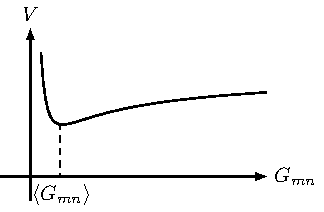
\includegraphics[keepaspectratio,width=0.8\linewidth]{fig/intro_potential/intro_potential.pdf}         
      \end{figure}
    \end{column}
  \end{columns}

\end{frame}

\subsection{背景磁場}

\begin{frame}[plain]
  \frametitle{\thesubsection.\ \subsecname}

  \citefone{Abe_SuperfieldDescription_2012}{H. Abe, T. Kobayashi, H. Ohki, and K. Sumita}{6}

  \vspace*{-10pt}

  真空期待値を次のように決める.
  \begin{equation}
    \ev*{A_{i}}
    =
    \frac{\pi}{\Im \tau_{i}}\textcolor{black}{M^{(i)}}\bar{z}_{i}
    ,
    \nonumber
  \end{equation}
  \begin{equation}
    \textcolor{black}{
      M^{(i)}
    }
    \textcolor{black}{
      =
      \begin{pmatrix}
        M_{1}^{(i)} &0 &\cdots & 0\\
        0&M_{2}^{(i)}&\cdots&0\\
        \vdots& \vdots& \ddots &\vdots \\
        0 & 0 & \cdots & M_{N}^{(i)}
      \end{pmatrix}
    }
    .
    \nonumber
  \end{equation}

  \begin{itemize}
    \color{black}
    \item 
    $M_{a}^{(i)}$は整数
    \item 
    $M^{(i)}$はトーラス上の磁場
    $\rightarrow$
    $F_{45}=\pi M^{(1)}$など
    \item 
    ブロック対角化でより小さいゲージ対称性

    \vspace*{-20pt}

    $$
      U(N)
      \rightarrow
      U(N_1)
      \times
      U(N_2)
      \times
      \cdots
      \times
      U(\tilde{N})
    $$
  \end{itemize}
  
\end{frame}


\subsection{参照点とモジュライ固定}

\begin{frame}[plain]
  \frametitle{\thesubsection.\ \subsecname}

  \citeftwo{Abe_ModuliStabilization_2007a}{H. Abe, T. Higaki, T. Kobayashi, and Y. Omura}{Abe_MoreFterm_2007a}{H. Abe, T. Higaki, and T. Kobayashi}{6}

  \begin{tikzpicture}[remember picture, overlay]
    \node[anchor=north east, align=left] at ($(current page.north east)-(0,5.4)$){
    {
      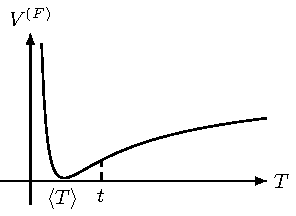
\includegraphics[keepaspectratio,width=2.5cm]{fig/reference_point/reference_point.pdf}       
    }
    };
  \end{tikzpicture}

  \vspace*{-1.5cm}

  \begin{itemize}
    \item 
    スーパーポテンシャル$W$とケーラーポテンシャル$K$

    \hspace{1cm}$\longrightarrow$スカラーポテンシャル(\textcolor{DarkRed}{$F$-termポテンシャル})
    \begin{gather}
      V^{(F)}
      \equiv
      e^{K}
      (
        K^{I\bar{J}}(D_{I}W)(D_{\bar{J}}\bar{W})
        -
        3|W|^2
      )
      \nonumber
      \\
      D_{I}W
      \equiv
      W_{I}+K_{I}W
      \quad
      (I=X,T)
      \nonumber
    \end{gather}
    \begin{center}
      $f_{I}\equiv\partial_{I}f$,$K^{I\bar{J}}$は$K_{I\bar{J}}$の逆行列      
    \end{center}
    \item 
    $V^{(F)}$の最小値を実現する$T,X$は?

    \hspace{2cm}$\longrightarrow$
    その点にモジュライ$T$が固定
  
    \item 
    ポテンシャルの最小をどのように特定するか?
  
    \begin{itemize}
      \item 
      解析的には難しい
      $\longrightarrow$
      \textcolor{DarkRed}{参照点}を利用すると解析的に
      \item 
      \textcolor{DarkMagenta}{超対称性が保たれる点}がポテンシャルの最小になりやすい
    \end{itemize}
  \end{itemize}
  
\end{frame}

\begin{frame}
  \frametitle{\thesubsection.\ \subsecname}

  \citefone{Abe_ModuliStabilization_2007a}{H. Abe, T. Higaki, T. Kobayashi, and Y. Omura}{6}

  \begin{itemize}
    \item 
    参照点$(t,x)$
    \begin{equation}
      \hspace*{-1cm}
      D_{T}W
      \left.\vphantom{\frac{1}{2}}\right|_{0}
      =0
      ,\ 
      V_{X}^{(F)}
      \left.\vphantom{\frac{1}{2}}\right|_{0}
      =0
      \quad
      (
        \text{
          $\left.\cdot\hspace{1pt}\right|_{0}$は$(T,X)=(t,x)$の代入
        }
      )
      \nonumber
    \end{equation}
    \begin{center}
      ($D_{T}W=0\longrightarrow$超対称性が保たれている)
    \end{center}
    \item 
    ポテンシャル$V^{(F)}$を参照点からの揺らぎ$\delta T,\delta X$で展開
    \begin{align}
      V^{(F)}
      &=
      \textcolor{gray}{
        V^{(F)}      
        \left.\vphantom{\frac{1}{2}}\right|_{0}
        +
      }
      V_{T}^{(F)}
      \left.\vphantom{\frac{1}{2}}\right|_{0}
      \delta T
      \textcolor{gray}{
        +
        V_{X}^{(F)}
        \left.\vphantom{\frac{1}{2}}\right|_{0}
        \delta X
        +
        \cdots
        +
      }
      \nonumber
      \\
      &\hspace{-5pt}
      +
      \frac{1}{2}
      V_{TT}^{(F)}
      \left.\vphantom{\frac{1}{2}}\right|_{0}
      \delta T^2
      +
      \frac{1}{2}
      V_{T\bar{T}}^{(F)}
      \left.\vphantom{\frac{1}{2}}\right|_{0}
      \delta T\delta \bar{T}
      +
      \cdots
      \nonumber
    \end{align}
  \end{itemize}

\end{frame}


\begin{frame}
  \frametitle{\thesubsection.\ \subsecname}

  $V_{\delta T}, V_{\delta \bar{T}}, V_{\delta X}, V_{\delta \bar{X}}=0\longrightarrow$
  $\delta T, \delta \bar{T}, \delta X, \delta \bar{X}$の値を決定
  \begin{center}
    {\LARGE $\downarrow$}
    
    $\displaystyle
      \frac{\delta T}{t}\ll 1
      ,\ 
      \frac{\delta X}{x}\ll 1
    $
    であれば,\textcolor{DarkRed}{参照点}による近似が有効
  \end{center}

\end{frame}


\subsection{モジュライ固定の例}

\begin{frame}[plain]
  \frametitle{\thesubsection.\ \subsecname}







  
\end{frame}

% \begin{frame}[plain]
%   \frametitle{\thesubsection\ \subsecname}







  
% \end{frame}

% --------------------------

\section{参考文献}
\begin{frame}[plain,allowframebreaks]
  \frametitle{\secname}
  \scriptsize
  \beamertemplatetextbibitems
  \bibliographystyle{ytphys}
  \bibliography{hoge}

  \nocite{Wess_SupersymmetrySupergravity_1992}

  \nocite{柴崎_背景_2021}
  \nocite{中野_磁化_2023}

\end{frame}


\setcounter{framenumber}{\value{Appendix}}
\end{document}
